\documentclass[1p]{elsarticle_modified}
%\bibliographystyle{elsarticle-num}

%\usepackage[colorlinks]{hyperref}
%\usepackage{abbrmath_seonhwa} %\Abb, \Ascr, \Acal ,\Abf, \Afrak
\usepackage{amsfonts}
\usepackage{amssymb}
\usepackage{amsmath}
\usepackage{amsthm}
\usepackage{scalefnt}
\usepackage{amsbsy}
\usepackage{kotex}
\usepackage{caption}
\usepackage{subfig}
\usepackage{color}
\usepackage{graphicx}
\usepackage{xcolor} %% white, black, red, green, blue, cyan, magenta, yellow
\usepackage{float}
\usepackage{setspace}
\usepackage{hyperref}

\usepackage{tikz}
\usetikzlibrary{arrows}

\usepackage{multirow}
\usepackage{array} % fixed length table
\usepackage{hhline}

%%%%%%%%%%%%%%%%%%%%%
\makeatletter
\renewcommand*\env@matrix[1][\arraystretch]{%
	\edef\arraystretch{#1}%
	\hskip -\arraycolsep
	\let\@ifnextchar\new@ifnextchar
	\array{*\c@MaxMatrixCols c}}
\makeatother %https://tex.stackexchange.com/questions/14071/how-can-i-increase-the-line-spacing-in-a-matrix
%%%%%%%%%%%%%%%

\usepackage[normalem]{ulem}

\newcommand{\msout}[1]{\ifmmode\text{\sout{\ensuremath{#1}}}\else\sout{#1}\fi}
%SOURCE: \msout is \stkout macro in https://tex.stackexchange.com/questions/20609/strikeout-in-math-mode

\newcommand{\cancel}[1]{
	\ifmmode
	{\color{red}\msout{#1}}
	\else
	{\color{red}\sout{#1}}
	\fi
}

\newcommand{\add}[1]{
	{\color{blue}\uwave{#1}}
}

\newcommand{\replace}[2]{
	\ifmmode
	{\color{red}\msout{#1}}{\color{blue}\uwave{#2}}
	\else
	{\color{red}\sout{#1}}{\color{blue}\uwave{#2}}
	\fi
}

\newcommand{\Sol}{\mathcal{S}} %segment
\newcommand{\D}{D} %diagram
\newcommand{\A}{\mathcal{A}} %arc


%%%%%%%%%%%%%%%%%%%%%%%%%%%%%5 test

\def\sl{\operatorname{\textup{SL}}(2,\Cbb)}
\def\psl{\operatorname{\textup{PSL}}(2,\Cbb)}
\def\quan{\mkern 1mu \triangleright \mkern 1mu}

\theoremstyle{definition}
\newtheorem{thm}{Theorem}[section]
\newtheorem{prop}[thm]{Proposition}
\newtheorem{lem}[thm]{Lemma}
\newtheorem{ques}[thm]{Question}
\newtheorem{cor}[thm]{Corollary}
\newtheorem{defn}[thm]{Definition}
\newtheorem{exam}[thm]{Example}
\newtheorem{rmk}[thm]{Remark}
\newtheorem{alg}[thm]{Algorithm}

\newcommand{\I}{\sqrt{-1}}
\begin{document}

%\begin{frontmatter}
%
%\title{Boundary parabolic representations of knots up to 8 crossings}
%
%%% Group authors per affiliation:
%\author{Yunhi Cho} 
%\address{Department of Mathematics, University of Seoul, Seoul, Korea}
%\ead{yhcho@uos.ac.kr}
%
%
%\author{Seonhwa Kim} %\fnref{s_kim}}
%\address{Center for Geometry and Physics, Institute for Basic Science, Pohang, 37673, Korea}
%\ead{ryeona17@ibs.re.kr}
%
%\author{Hyuk Kim}
%\address{Department of Mathematical Sciences, Seoul National University, Seoul 08826, Korea}
%\ead{hyukkim@snu.ac.kr}
%
%\author{Seokbeom Yoon}
%\address{Department of Mathematical Sciences, Seoul National University, Seoul, 08826,  Korea}
%\ead{sbyoon15@snu.ac.kr}
%
%\begin{abstract}
%We find all boundary parabolic representation of knots up to 8 crossings.
%
%\end{abstract}
%\begin{keyword}
%    \MSC[2010] 57M25 
%\end{keyword}
%
%\end{frontmatter}

%\linenumbers
%\tableofcontents
%
\newcommand\colored[1]{\textcolor{white}{\rule[-0.35ex]{0.8em}{1.4ex}}\kern-0.8em\color{red} #1}%
%\newcommand\colored[1]{\textcolor{white}{ #1}\kern-2.17ex	\textcolor{white}{ #1}\kern-1.81ex	\textcolor{white}{ #1}\kern-2.15ex\color{red}#1	}

{\Large $\underline{12n_{0433}~(K12n_{0433})}$}

\setlength{\tabcolsep}{10pt}
\renewcommand{\arraystretch}{1.6}
\vspace{1cm}\begin{tabular}{m{100pt}>{\centering\arraybackslash}m{274pt}}
\multirow{5}{120pt}{
	\centering
	\includegraphics[width=112pt]{../../../GIT/diagram.site/Diagrams/png/2522_12n_0433.png}\\
\ \ \ A knot diagram\footnotemark}&
\allowdisplaybreaks
\textbf{Linearized knot diagam} \\
\cline{2-2}
 &
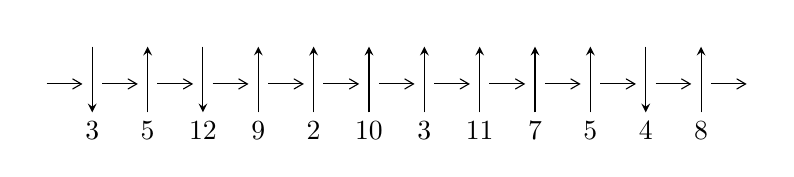
\begin{tikzpicture}[x=20pt, y=17pt]
	% nodes
	\node (C0) at (0, 0) {};
	\node (C1) at (1, 0) {};
	\node (C1U) at (1, +1) {};
	\node (C1D) at (1, -1) {3};

	\node (C2) at (2, 0) {};
	\node (C2U) at (2, +1) {};
	\node (C2D) at (2, -1) {5};

	\node (C3) at (3, 0) {};
	\node (C3U) at (3, +1) {};
	\node (C3D) at (3, -1) {12};

	\node (C4) at (4, 0) {};
	\node (C4U) at (4, +1) {};
	\node (C4D) at (4, -1) {9};

	\node (C5) at (5, 0) {};
	\node (C5U) at (5, +1) {};
	\node (C5D) at (5, -1) {2};

	\node (C6) at (6, 0) {};
	\node (C6U) at (6, +1) {};
	\node (C6D) at (6, -1) {10};

	\node (C7) at (7, 0) {};
	\node (C7U) at (7, +1) {};
	\node (C7D) at (7, -1) {3};

	\node (C8) at (8, 0) {};
	\node (C8U) at (8, +1) {};
	\node (C8D) at (8, -1) {11};

	\node (C9) at (9, 0) {};
	\node (C9U) at (9, +1) {};
	\node (C9D) at (9, -1) {7};

	\node (C10) at (10, 0) {};
	\node (C10U) at (10, +1) {};
	\node (C10D) at (10, -1) {5};

	\node (C11) at (11, 0) {};
	\node (C11U) at (11, +1) {};
	\node (C11D) at (11, -1) {4};

	\node (C12) at (12, 0) {};
	\node (C12U) at (12, +1) {};
	\node (C12D) at (12, -1) {8};
	\node (C13) at (13, 0) {};

	% arrows
	\draw[->,>={angle 60}]
	(C0) edge (C1) (C1) edge (C2) (C2) edge (C3) (C3) edge (C4) (C4) edge (C5) (C5) edge (C6) (C6) edge (C7) (C7) edge (C8) (C8) edge (C9) (C9) edge (C10) (C10) edge (C11) (C11) edge (C12) (C12) edge (C13) ;	\draw[->,>=stealth]
	(C1U) edge (C1D) (C2D) edge (C2U) (C3U) edge (C3D) (C4D) edge (C4U) (C5D) edge (C5U) (C6D) edge (C6U) (C7D) edge (C7U) (C8D) edge (C8U) (C9D) edge (C9U) (C10D) edge (C10U) (C11U) edge (C11D) (C12D) edge (C12U) ;
	\end{tikzpicture} \\
\hhline{~~} \\& 
\textbf{Solving Sequence} \\ \cline{2-2} 
 &
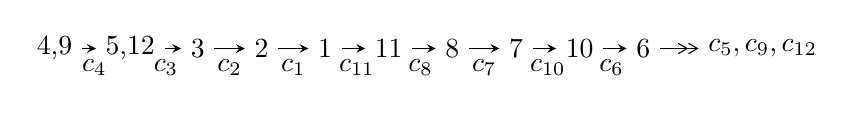
\begin{tikzpicture}[x=23pt, y=7pt]
	% node
	\node (A0) at (-1/8, 0) {4,9};
	\node (A1) at (17/16, 0) {5,12};
	\node (A2) at (17/8, 0) {3};
	\node (A3) at (25/8, 0) {2};
	\node (A4) at (33/8, 0) {1};
	\node (A5) at (41/8, 0) {11};
	\node (A6) at (49/8, 0) {8};
	\node (A7) at (57/8, 0) {7};
	\node (A8) at (65/8, 0) {10};
	\node (A9) at (73/8, 0) {6};
	\node (C1) at (1/2, -1) {$c_{4}$};
	\node (C2) at (13/8, -1) {$c_{3}$};
	\node (C3) at (21/8, -1) {$c_{2}$};
	\node (C4) at (29/8, -1) {$c_{1}$};
	\node (C5) at (37/8, -1) {$c_{11}$};
	\node (C6) at (45/8, -1) {$c_{8}$};
	\node (C7) at (53/8, -1) {$c_{7}$};
	\node (C8) at (61/8, -1) {$c_{10}$};
	\node (C9) at (69/8, -1) {$c_{6}$};
	\node (A10) at (11, 0) {$c_{5},c_{9},c_{12}$};

	% edge
	\draw[->,>=stealth]	
	(A0) edge (A1) (A1) edge (A2) (A2) edge (A3) (A3) edge (A4) (A4) edge (A5) (A5) edge (A6) (A6) edge (A7) (A7) edge (A8) (A8) edge (A9) ;
	\draw[->>,>={angle 60}]	
	(A9) edge (A10);
\end{tikzpicture} \\ 

\end{tabular} \\

\footnotetext{
The image of knot diagram is generated by the software ``\textbf{Draw programme}" developed by Andrew Bartholomew(\url{http://www.layer8.co.uk/maths/draw/index.htm\#Running-draw}), where we modified some parts for our purpose(\url{https://github.com/CATsTAILs/LinksPainter}).
}\phantom \\ \newline 
\centering \textbf{Ideals for irreducible components\footnotemark of $X_{\text{par}}$} 
 
\begin{align*}
I^u_{1}&=\langle 
-4 u^{18}-56 u^{17}+\cdots+4 b+144,\;9 u^{18}+116 u^{17}+\cdots+8 a-144,\;u^{19}+14 u^{18}+\cdots-176 u-32\rangle \\
I^u_{2}&=\langle 
u^{12}-2 u^{11}-2 u^{10}+8 u^9- u^8-14 u^7+10 u^6+13 u^5-15 u^4-5 u^3+11 u^2+b-3,\\
\phantom{I^u_{2}}&\phantom{= \langle  }4 u^{13}-8 u^{12}-7 u^{11}+30 u^{10}-6 u^9-48 u^8+39 u^7+38 u^6-50 u^5-11 u^4+32 u^3- u^2+a-8 u,\\
\phantom{I^u_{2}}&\phantom{= \langle  }u^{14}-2 u^{13}-2 u^{12}+8 u^{11}- u^{10}-14 u^9+10 u^8+13 u^7-15 u^6-6 u^5+12 u^4+u^3-5 u^2+1\rangle \\
\\
\end{align*}
\raggedright * 2 irreducible components of $\dim_{\mathbb{C}}=0$, with total 33 representations.\\
\footnotetext{All coefficients of polynomials are rational numbers. But the coefficients are sometimes approximated in decimal forms when there is not enough margin.}
\newpage
\renewcommand{\arraystretch}{1}
\centering \section*{I. $I^u_{1}= \langle -4 u^{18}-56 u^{17}+\cdots+4 b+144,\;9 u^{18}+116 u^{17}+\cdots+8 a-144,\;u^{19}+14 u^{18}+\cdots-176 u-32 \rangle$}
\flushleft \textbf{(i) Arc colorings}\\
\begin{tabular}{m{7pt} m{180pt} m{7pt} m{180pt} }
\flushright $a_{4}=$&$\begin{pmatrix}1\\0\end{pmatrix}$ \\
\flushright $a_{9}=$&$\begin{pmatrix}0\\u\end{pmatrix}$ \\
\flushright $a_{5}=$&$\begin{pmatrix}1\\- u^2\end{pmatrix}$ \\
\flushright $a_{12}=$&$\begin{pmatrix}-\frac{9}{8} u^{18}-\frac{29}{2} u^{17}+\cdots+\frac{397}{4} u+18\\u^{18}+14 u^{17}+\cdots-175 u-36\end{pmatrix}$ \\
\flushright $a_{3}=$&$\begin{pmatrix}-\frac{3}{2} u^{18}-\frac{353}{16} u^{17}+\cdots+400 u+89\\-\frac{43}{16} u^{18}-35 u^{17}+\cdots+284 u+52\end{pmatrix}$ \\
\flushright $a_{2}=$&$\begin{pmatrix}-\frac{47}{16} u^{18}-\frac{617}{16} u^{17}+\cdots+351 u+71\\\frac{33}{16} u^{18}+\frac{55}{2} u^{17}+\cdots-308 u-64\end{pmatrix}$ \\
\flushright $a_{1}=$&$\begin{pmatrix}-3 u^{18}-\frac{75}{2} u^{17}+\cdots+179 u+\frac{59}{2}\\\frac{7}{2} u^{18}+47 u^{17}+\cdots-\frac{931}{2} u-92\end{pmatrix}$ \\
\flushright $a_{11}=$&$\begin{pmatrix}-\frac{1}{8} u^{18}-\frac{1}{2} u^{17}+\cdots-\frac{303}{4} u-18\\u^{18}+14 u^{17}+\cdots-175 u-36\end{pmatrix}$ \\
\flushright $a_{8}=$&$\begin{pmatrix}-\frac{37}{8} u^{18}-\frac{879}{16} u^{17}+\cdots-18 u-28\\\frac{25}{16} u^{18}+\frac{99}{4} u^{17}+\cdots-596 u-134\end{pmatrix}$ \\
\flushright $a_{7}=$&$\begin{pmatrix}-\frac{1}{8} u^{18}-\frac{3}{2} u^{17}+\cdots+\frac{3}{2} u-\frac{1}{2}\\\frac{1}{4} u^{18}+\frac{13}{4} u^{17}+\cdots-\frac{43}{2} u-4\end{pmatrix}$ \\
\flushright $a_{10}=$&$\begin{pmatrix}\frac{9}{8} u^{18}+\frac{59}{4} u^{17}+\cdots-\frac{467}{4} u-22\\-\frac{5}{4} u^{18}-17 u^{17}+\cdots+181 u+36\end{pmatrix}$ \\
\flushright $a_{6}=$&$\begin{pmatrix}-0.812500 u^{18}-13.1250 u^{17}+\cdots+309.500 u+67.5000\\-\frac{1}{4} u^{18}-\frac{7}{8} u^{17}+\cdots-\frac{413}{2} u-50\end{pmatrix}$\\&\end{tabular}
\flushleft \textbf{(ii) Obstruction class $= -1$}\\~\\
\flushleft \textbf{(iii) Cusp Shapes $= \frac{11}{2} u^{18}+\frac{139}{2} u^{17}+415 u^{16}+1500 u^{15}+\frac{7043}{2} u^{14}+\frac{10513}{2} u^{13}+4038 u^{12}-\frac{2097}{2} u^{11}-5824 u^{10}-\frac{8859}{2} u^9+2557 u^8+\frac{15599}{2} u^7+6701 u^6+\frac{4531}{2} u^5-\frac{1461}{2} u^4-\frac{2433}{2} u^3-610 u^2-104 u+26$}\\~\\
\newpage\renewcommand{\arraystretch}{1}
\flushleft \textbf{(iv) u-Polynomials at the component}\newline \\
\begin{tabular}{m{50pt}|m{274pt}}
Crossings & \hspace{64pt}u-Polynomials at each crossing \\
\hline $$\begin{aligned}c_{1}\end{aligned}$$&$\begin{aligned}
&u^{19}+52 u^{18}+\cdots+153907 u-11881
\end{aligned}$\\
\hline $$\begin{aligned}c_{2},c_{5}\end{aligned}$$&$\begin{aligned}
&u^{19}+2 u^{18}+\cdots+251 u-109
\end{aligned}$\\
\hline $$\begin{aligned}c_{3},c_{11}\end{aligned}$$&$\begin{aligned}
&u^{19}-3 u^{18}+\cdots+6 u-1
\end{aligned}$\\
\hline $$\begin{aligned}c_{4}\end{aligned}$$&$\begin{aligned}
&u^{19}+14 u^{18}+\cdots-176 u-32
\end{aligned}$\\
\hline $$\begin{aligned}c_{6},c_{9}\end{aligned}$$&$\begin{aligned}
&u^{19}+3 u^{18}+\cdots+5 u-1
\end{aligned}$\\
\hline $$\begin{aligned}c_{7}\end{aligned}$$&$\begin{aligned}
&u^{19}+6 u^{18}+\cdots-10302 u-2521
\end{aligned}$\\
\hline $$\begin{aligned}c_{8}\end{aligned}$$&$\begin{aligned}
&u^{19}+7 u^{18}+\cdots+162 u-297
\end{aligned}$\\
\hline $$\begin{aligned}c_{10}\end{aligned}$$&$\begin{aligned}
&u^{19}- u^{18}+\cdots+34163 u-22951
\end{aligned}$\\
\hline $$\begin{aligned}c_{12}\end{aligned}$$&$\begin{aligned}
&u^{19}- u^{18}+\cdots+2 u-1
\end{aligned}$\\
\hline
\end{tabular}\\~\\
\newpage\renewcommand{\arraystretch}{1}
\flushleft \textbf{(v) Riley Polynomials at the component}\newline \\
\begin{tabular}{m{50pt}|m{274pt}}
Crossings & \hspace{64pt}Riley Polynomials at each crossing \\
\hline $$\begin{aligned}c_{1}\end{aligned}$$&$\begin{aligned}
&y^{19}-304 y^{18}+\cdots+28531319635 y-141158161
\end{aligned}$\\
\hline $$\begin{aligned}c_{2},c_{5}\end{aligned}$$&$\begin{aligned}
&y^{19}+52 y^{18}+\cdots+153907 y-11881
\end{aligned}$\\
\hline $$\begin{aligned}c_{3},c_{11}\end{aligned}$$&$\begin{aligned}
&y^{19}+13 y^{18}+\cdots+18 y-1
\end{aligned}$\\
\hline $$\begin{aligned}c_{4}\end{aligned}$$&$\begin{aligned}
&y^{19}-8 y^{18}+\cdots+2816 y-1024
\end{aligned}$\\
\hline $$\begin{aligned}c_{6},c_{9}\end{aligned}$$&$\begin{aligned}
&y^{19}+45 y^{18}+\cdots-13 y-1
\end{aligned}$\\
\hline $$\begin{aligned}c_{7}\end{aligned}$$&$\begin{aligned}
&y^{19}+78 y^{18}+\cdots-54658176 y-6355441
\end{aligned}$\\
\hline $$\begin{aligned}c_{8}\end{aligned}$$&$\begin{aligned}
&y^{19}+3 y^{18}+\cdots+334530 y-88209
\end{aligned}$\\
\hline $$\begin{aligned}c_{10}\end{aligned}$$&$\begin{aligned}
&y^{19}+111 y^{18}+\cdots+3474236893 y-526748401
\end{aligned}$\\
\hline $$\begin{aligned}c_{12}\end{aligned}$$&$\begin{aligned}
&y^{19}+47 y^{18}+\cdots+6 y-1
\end{aligned}$\\
\hline
\end{tabular}\\~\\
\newpage\flushleft \textbf{(vi) Complex Volumes and Cusp Shapes}
$$\begin{array}{c|c|c}  
\text{Solutions to }I^u_{1}& \I (\text{vol} + \sqrt{-1}CS) & \text{Cusp shape}\\
 \hline 
\begin{aligned}
u &= \phantom{-}0.952043 + 0.382374 I \\
a &= \phantom{-}1.17972 + 1.64280 I \\
b &= \phantom{-}0.089418 - 1.147290 I\end{aligned}
 & \phantom{-}3.73582 + 1.17440 I & \phantom{-}11.92191 - 0.82107 I \\ \hline\begin{aligned}
u &= \phantom{-}0.952043 - 0.382374 I \\
a &= \phantom{-}1.17972 - 1.64280 I \\
b &= \phantom{-}0.089418 + 1.147290 I\end{aligned}
 & \phantom{-}3.73582 - 1.17440 I & \phantom{-}11.92191 + 0.82107 I \\ \hline\begin{aligned}
u &= -0.768934 + 0.440549 I \\
a &= \phantom{-}0.024948 + 0.607572 I \\
b &= -0.703023 - 0.273400 I\end{aligned}
 & -1.08916 - 1.88825 I & \phantom{-}4.12654 + 6.95874 I \\ \hline\begin{aligned}
u &= -0.768934 - 0.440549 I \\
a &= \phantom{-}0.024948 - 0.607572 I \\
b &= -0.703023 + 0.273400 I\end{aligned}
 & -1.08916 + 1.88825 I & \phantom{-}4.12654 - 6.95874 I \\ \hline\begin{aligned}
u &= -0.843250 + 0.773517 I \\
a &= \phantom{-}0.454480 - 0.127733 I \\
b &= \phantom{-}0.322216 - 0.786249 I\end{aligned}
 & -2.76916 - 1.41416 I & \phantom{-}5.64379 - 1.17536 I \\ \hline\begin{aligned}
u &= -0.843250 - 0.773517 I \\
a &= \phantom{-}0.454480 + 0.127733 I \\
b &= \phantom{-}0.322216 + 0.786249 I\end{aligned}
 & -2.76916 + 1.41416 I & \phantom{-}5.64379 + 1.17536 I \\ \hline\begin{aligned}
u &= -0.909852 + 0.767638 I \\
a &= \phantom{-}1.56617 - 0.42091 I \\
b &= \phantom{-}0.328613 + 0.853253 I\end{aligned}
 & -2.57134 - 4.39733 I & \phantom{-}2.20465 + 4.40914 I \\ \hline\begin{aligned}
u &= -0.909852 - 0.767638 I \\
a &= \phantom{-}1.56617 + 0.42091 I \\
b &= \phantom{-}0.328613 - 0.853253 I\end{aligned}
 & -2.57134 + 4.39733 I & \phantom{-}2.20465 - 4.40914 I \\ \hline\begin{aligned}
u &= -1.144960 + 0.452451 I \\
a &= -0.86753 + 1.89248 I \\
b &= -0.425367 - 1.315850 I\end{aligned}
 & \phantom{-}3.58710 - 6.01331 I & \phantom{-}10.19213 + 3.01505 I \\ \hline\begin{aligned}
u &= -1.144960 - 0.452451 I \\
a &= -0.86753 - 1.89248 I \\
b &= -0.425367 + 1.315850 I\end{aligned}
 & \phantom{-}3.58710 + 6.01331 I & \phantom{-}10.19213 - 3.01505 I\\
 \hline 
 \end{array}$$\newpage$$\begin{array}{c|c|c}  
\text{Solutions to }I^u_{1}& \I (\text{vol} + \sqrt{-1}CS) & \text{Cusp shape}\\
 \hline 
\begin{aligned}
u &= -0.139548 + 0.627235 I \\
a &= -0.010591 - 0.198980 I \\
b &= -0.307852 + 1.015400 I\end{aligned}
 & \phantom{-}0.72950 + 1.86007 I & \phantom{-}4.96965 - 3.09776 I \\ \hline\begin{aligned}
u &= -0.139548 - 0.627235 I \\
a &= -0.010591 + 0.198980 I \\
b &= -0.307852 - 1.015400 I\end{aligned}
 & \phantom{-}0.72950 - 1.86007 I & \phantom{-}4.96965 + 3.09776 I \\ \hline\begin{aligned}
u &= \phantom{-}0.583970\phantom{ +0.000000I} \\
a &= \phantom{-}0.561976\phantom{ +0.000000I} \\
b &= \phantom{-}0.210478\phantom{ +0.000000I}\end{aligned}
 & \phantom{-}0.754048\phantom{ +0.000000I} & \phantom{-}13.8110\phantom{ +0.000000I} \\ \hline\begin{aligned}
u &= -1.46571 + 1.27783 I \\
a &= \phantom{-}0.081435 - 0.340297 I \\
b &= \phantom{-}1.048890 - 0.034516 I\end{aligned}
 & \phantom{-}17.0824 - 5.1917 I & \phantom{-}2.96217 + 1.77524 I \\ \hline\begin{aligned}
u &= -1.46571 - 1.27783 I \\
a &= \phantom{-}0.081435 + 0.340297 I \\
b &= \phantom{-}1.048890 + 0.034516 I\end{aligned}
 & \phantom{-}17.0824 + 5.1917 I & \phantom{-}2.96217 - 1.77524 I \\ \hline\begin{aligned}
u &= -1.42781 + 1.33926 I \\
a &= \phantom{-}0.98158 - 1.30284 I \\
b &= \phantom{-}0.54039 + 1.33382 I\end{aligned}
 & -18.3616 - 10.8389 I & \phantom{-}6.00000 + 4.45622 I \\ \hline\begin{aligned}
u &= -1.42781 - 1.33926 I \\
a &= \phantom{-}0.98158 + 1.30284 I \\
b &= \phantom{-}0.54039 - 1.33382 I\end{aligned}
 & -18.3616 + 10.8389 I & \phantom{-}6.00000 - 4.45622 I \\ \hline\begin{aligned}
u &= -1.54397 + 1.24729 I \\
a &= \phantom{-}0.058807 + 1.056090 I \\
b &= \phantom{-}0.50147 - 1.36952 I\end{aligned}
 & -17.9924 + 0.3271 I & \phantom{-}6.00000 + 0. I\phantom{ +0.000000I} \\ \hline\begin{aligned}
u &= -1.54397 - 1.24729 I \\
a &= \phantom{-}0.058807 - 1.056090 I \\
b &= \phantom{-}0.50147 + 1.36952 I\end{aligned}
 & -17.9924 - 0.3271 I & \phantom{-}6.00000 + 0. I\phantom{ +0.000000I}\\
 \hline 
 \end{array}$$\newpage\newpage\renewcommand{\arraystretch}{1}
\centering \section*{II. $I^u_{2}= \langle u^{12}-2 u^{11}+\cdots+b-3,\;4 u^{13}-8 u^{12}+\cdots+a-8 u,\;u^{14}-2 u^{13}+\cdots-5 u^2+1 \rangle$}
\flushleft \textbf{(i) Arc colorings}\\
\begin{tabular}{m{7pt} m{180pt} m{7pt} m{180pt} }
\flushright $a_{4}=$&$\begin{pmatrix}1\\0\end{pmatrix}$ \\
\flushright $a_{9}=$&$\begin{pmatrix}0\\u\end{pmatrix}$ \\
\flushright $a_{5}=$&$\begin{pmatrix}1\\- u^2\end{pmatrix}$ \\
\flushright $a_{12}=$&$\begin{pmatrix}-4 u^{13}+8 u^{12}+\cdots+u^2+8 u\\- u^{12}+2 u^{11}+\cdots-11 u^2+3\end{pmatrix}$ \\
\flushright $a_{3}=$&$\begin{pmatrix}u^{13}- u^{12}+\cdots+4 u-3\\u^{13}- u^{12}+\cdots-4 u+1\end{pmatrix}$ \\
\flushright $a_{2}=$&$\begin{pmatrix}-2 u^{13}+4 u^{12}+\cdots+9 u-3\\2 u^{13}-2 u^{12}+\cdots+6 u^2-7 u\end{pmatrix}$ \\
\flushright $a_{1}=$&$\begin{pmatrix}- u^{13}+2 u^{12}+\cdots-4 u-6\\2 u^{13}-4 u^{12}+\cdots-6 u-1\end{pmatrix}$ \\
\flushright $a_{11}=$&$\begin{pmatrix}-4 u^{13}+7 u^{12}+\cdots+8 u+3\\- u^{12}+2 u^{11}+\cdots-11 u^2+3\end{pmatrix}$ \\
\flushright $a_{8}=$&$\begin{pmatrix}7 u^{13}-9 u^{12}+\cdots-8 u-7\\2 u^{13}-2 u^{12}+\cdots-2 u-2\end{pmatrix}$ \\
\flushright $a_{7}=$&$\begin{pmatrix}- u^{12}+2 u^{11}+\cdots- u+4\\- u^{13}+2 u^{12}+\cdots-12 u^3+5 u\end{pmatrix}$ \\
\flushright $a_{10}=$&$\begin{pmatrix}-3 u^{13}+6 u^{12}+\cdots+4 u-1\\- u^{12}+2 u^{11}+\cdots+u+4\end{pmatrix}$ \\
\flushright $a_{6}=$&$\begin{pmatrix}u^{13}-5 u^{12}+\cdots-2 u+5\\-4 u^{13}+8 u^{12}+\cdots+9 u+1\end{pmatrix}$\\&\end{tabular}
\flushleft \textbf{(ii) Obstruction class $= 1$}\\~\\
\flushleft \textbf{(iii) Cusp Shapes $= -12 u^{13}+29 u^{12}+8 u^{11}-92 u^{10}+58 u^9+113 u^8-161 u^7-41 u^6+159 u^5-34 u^4-82 u^3+30 u^2+15 u-6$}\\~\\
\newpage\renewcommand{\arraystretch}{1}
\flushleft \textbf{(iv) u-Polynomials at the component}\newline \\
\begin{tabular}{m{50pt}|m{274pt}}
Crossings & \hspace{64pt}u-Polynomials at each crossing \\
\hline $$\begin{aligned}c_{1}\end{aligned}$$&$\begin{aligned}
&u^{14}-9 u^{13}+\cdots-4 u+1
\end{aligned}$\\
\hline $$\begin{aligned}c_{2}\end{aligned}$$&$\begin{aligned}
&u^{14}+u^{13}+\cdots+2 u^2+1
\end{aligned}$\\
\hline $$\begin{aligned}c_{3}\end{aligned}$$&$\begin{aligned}
&u^{14}+4 u^{13}+\cdots+5 u+1
\end{aligned}$\\
\hline $$\begin{aligned}c_{4}\end{aligned}$$&$\begin{aligned}
&u^{14}-2 u^{13}+\cdots-5 u^2+1
\end{aligned}$\\
\hline $$\begin{aligned}c_{5}\end{aligned}$$&$\begin{aligned}
&u^{14}- u^{13}+\cdots+2 u^2+1
\end{aligned}$\\
\hline $$\begin{aligned}c_{6}\end{aligned}$$&$\begin{aligned}
&u^{14}+2 u^{13}+\cdots+4 u^2+1
\end{aligned}$\\
\hline $$\begin{aligned}c_{7}\end{aligned}$$&$\begin{aligned}
&u^{14}+5 u^{13}+\cdots+25 u+31
\end{aligned}$\\
\hline $$\begin{aligned}c_{8}\end{aligned}$$&$\begin{aligned}
&u^{14}+2 u^{13}+\cdots+5 u+1
\end{aligned}$\\
\hline $$\begin{aligned}c_{9}\end{aligned}$$&$\begin{aligned}
&u^{14}-2 u^{13}+\cdots+4 u^2+1
\end{aligned}$\\
\hline $$\begin{aligned}c_{10}\end{aligned}$$&$\begin{aligned}
&u^{14}-4 u^{13}+\cdots-136 u+31
\end{aligned}$\\
\hline $$\begin{aligned}c_{11}\end{aligned}$$&$\begin{aligned}
&u^{14}-4 u^{13}+\cdots-5 u+1
\end{aligned}$\\
\hline $$\begin{aligned}c_{12}\end{aligned}$$&$\begin{aligned}
&u^{14}+4 u^{12}+\cdots- u+1
\end{aligned}$\\
\hline
\end{tabular}\\~\\
\newpage\renewcommand{\arraystretch}{1}
\flushleft \textbf{(v) Riley Polynomials at the component}\newline \\
\begin{tabular}{m{50pt}|m{274pt}}
Crossings & \hspace{64pt}Riley Polynomials at each crossing \\
\hline $$\begin{aligned}c_{1}\end{aligned}$$&$\begin{aligned}
&y^{14}-7 y^{13}+\cdots+8 y+1
\end{aligned}$\\
\hline $$\begin{aligned}c_{2},c_{5}\end{aligned}$$&$\begin{aligned}
&y^{14}+9 y^{13}+\cdots+4 y+1
\end{aligned}$\\
\hline $$\begin{aligned}c_{3},c_{11}\end{aligned}$$&$\begin{aligned}
&y^{14}+10 y^{13}+\cdots+5 y+1
\end{aligned}$\\
\hline $$\begin{aligned}c_{4}\end{aligned}$$&$\begin{aligned}
&y^{14}-8 y^{13}+\cdots-10 y+1
\end{aligned}$\\
\hline $$\begin{aligned}c_{6},c_{9}\end{aligned}$$&$\begin{aligned}
&y^{14}+10 y^{13}+\cdots+8 y+1
\end{aligned}$\\
\hline $$\begin{aligned}c_{7}\end{aligned}$$&$\begin{aligned}
&y^{14}+7 y^{13}+\cdots-1121 y+961
\end{aligned}$\\
\hline $$\begin{aligned}c_{8}\end{aligned}$$&$\begin{aligned}
&y^{14}-4 y^{13}+\cdots+17 y+1
\end{aligned}$\\
\hline $$\begin{aligned}c_{10}\end{aligned}$$&$\begin{aligned}
&y^{14}+12 y^{12}+\cdots+4506 y+961
\end{aligned}$\\
\hline $$\begin{aligned}c_{12}\end{aligned}$$&$\begin{aligned}
&y^{14}+8 y^{13}+\cdots+9 y+1
\end{aligned}$\\
\hline
\end{tabular}\\~\\
\newpage\flushleft \textbf{(vi) Complex Volumes and Cusp Shapes}
$$\begin{array}{c|c|c}  
\text{Solutions to }I^u_{2}& \I (\text{vol} + \sqrt{-1}CS) & \text{Cusp shape}\\
 \hline 
\begin{aligned}
u &= \phantom{-}0.798159 + 0.600990 I \\
a &= -0.790082 - 0.362242 I \\
b &= -0.292748 - 0.333907 I\end{aligned}
 & -3.42318 + 2.23744 I & \phantom{-}0.58128 - 4.57069 I \\ \hline\begin{aligned}
u &= \phantom{-}0.798159 - 0.600990 I \\
a &= -0.790082 + 0.362242 I \\
b &= -0.292748 + 0.333907 I\end{aligned}
 & -3.42318 - 2.23744 I & \phantom{-}0.58128 + 4.57069 I \\ \hline\begin{aligned}
u &= -0.869190 + 0.330016 I \\
a &= \phantom{-}0.409278 + 0.565077 I \\
b &= -0.984587 - 0.187907 I\end{aligned}
 & -1.77974 - 1.42720 I & -4.12456 + 2.68600 I \\ \hline\begin{aligned}
u &= -0.869190 - 0.330016 I \\
a &= \phantom{-}0.409278 - 0.565077 I \\
b &= -0.984587 + 0.187907 I\end{aligned}
 & -1.77974 + 1.42720 I & -4.12456 - 2.68600 I \\ \hline\begin{aligned}
u &= -1.127530 + 0.373386 I \\
a &= -0.63714 + 1.99005 I \\
b &= -0.46500 - 1.41759 I\end{aligned}
 & \phantom{-}3.27521 - 6.65870 I & \phantom{-}5.6824 + 13.1355 I \\ \hline\begin{aligned}
u &= -1.127530 - 0.373386 I \\
a &= -0.63714 - 1.99005 I \\
b &= -0.46500 + 1.41759 I\end{aligned}
 & \phantom{-}3.27521 + 6.65870 I & \phantom{-}5.6824 - 13.1355 I \\ \hline\begin{aligned}
u &= \phantom{-}0.723669 + 0.967507 I \\
a &= -1.268080 - 0.320652 I \\
b &= -0.228992 + 1.096290 I\end{aligned}
 & -1.31334 + 4.66687 I & \phantom{-}7.87120 - 4.64100 I \\ \hline\begin{aligned}
u &= \phantom{-}0.723669 - 0.967507 I \\
a &= -1.268080 + 0.320652 I \\
b &= -0.228992 - 1.096290 I\end{aligned}
 & -1.31334 - 4.66687 I & \phantom{-}7.87120 + 4.64100 I \\ \hline\begin{aligned}
u &= \phantom{-}0.726149 + 0.195111 I \\
a &= \phantom{-}1.18627 - 1.30389 I \\
b &= \phantom{-}0.445991 - 0.709258 I\end{aligned}
 & -4.05990 + 1.94786 I & -0.25504 - 3.63553 I \\ \hline\begin{aligned}
u &= \phantom{-}0.726149 - 0.195111 I \\
a &= \phantom{-}1.18627 + 1.30389 I \\
b &= \phantom{-}0.445991 + 0.709258 I\end{aligned}
 & -4.05990 - 1.94786 I & -0.25504 + 3.63553 I\\
 \hline 
 \end{array}$$\newpage$$\begin{array}{c|c|c}  
\text{Solutions to }I^u_{2}& \I (\text{vol} + \sqrt{-1}CS) & \text{Cusp shape}\\
 \hline 
\begin{aligned}
u &= -0.623048 + 0.243830 I \\
a &= \phantom{-}0.47491 - 1.88602 I \\
b &= -0.523041 + 1.186810 I\end{aligned}
 & \phantom{-}1.24309 + 3.87948 I & \phantom{-}3.25202 - 4.11136 I \\ \hline\begin{aligned}
u &= -0.623048 - 0.243830 I \\
a &= \phantom{-}0.47491 + 1.88602 I \\
b &= -0.523041 - 1.186810 I\end{aligned}
 & \phantom{-}1.24309 - 3.87948 I & \phantom{-}3.25202 + 4.11136 I \\ \hline\begin{aligned}
u &= \phantom{-}1.37179 + 0.58461 I \\
a &= \phantom{-}0.12484 + 1.47757 I \\
b &= \phantom{-}0.048376 - 1.236450 I\end{aligned}
 & \phantom{-}1.12307 + 2.18465 I & \phantom{-}7.49268 - 1.60290 I \\ \hline\begin{aligned}
u &= \phantom{-}1.37179 - 0.58461 I \\
a &= \phantom{-}0.12484 - 1.47757 I \\
b &= \phantom{-}0.048376 + 1.236450 I\end{aligned}
 & \phantom{-}1.12307 - 2.18465 I & \phantom{-}7.49268 + 1.60290 I\\
 \hline 
 \end{array}$$\newpage
\newpage\renewcommand{\arraystretch}{1}
\centering \section*{ III. u-Polynomials}
\begin{tabular}{m{50pt}|m{274pt}}
Crossings & \hspace{64pt}u-Polynomials at each crossing \\
\hline $$\begin{aligned}c_{1}\end{aligned}$$&$\begin{aligned}
&(u^{14}-9 u^{13}+\cdots-4 u+1)(u^{19}+52 u^{18}+\cdots+153907 u-11881)
\end{aligned}$\\
\hline $$\begin{aligned}c_{2}\end{aligned}$$&$\begin{aligned}
&(u^{14}+u^{13}+\cdots+2 u^2+1)(u^{19}+2 u^{18}+\cdots+251 u-109)
\end{aligned}$\\
\hline $$\begin{aligned}c_{3}\end{aligned}$$&$\begin{aligned}
&(u^{14}+4 u^{13}+\cdots+5 u+1)(u^{19}-3 u^{18}+\cdots+6 u-1)
\end{aligned}$\\
\hline $$\begin{aligned}c_{4}\end{aligned}$$&$\begin{aligned}
&(u^{14}-2 u^{13}+\cdots-5 u^2+1)(u^{19}+14 u^{18}+\cdots-176 u-32)
\end{aligned}$\\
\hline $$\begin{aligned}c_{5}\end{aligned}$$&$\begin{aligned}
&(u^{14}- u^{13}+\cdots+2 u^2+1)(u^{19}+2 u^{18}+\cdots+251 u-109)
\end{aligned}$\\
\hline $$\begin{aligned}c_{6}\end{aligned}$$&$\begin{aligned}
&(u^{14}+2 u^{13}+\cdots+4 u^2+1)(u^{19}+3 u^{18}+\cdots+5 u-1)
\end{aligned}$\\
\hline $$\begin{aligned}c_{7}\end{aligned}$$&$\begin{aligned}
&(u^{14}+5 u^{13}+\cdots+25 u+31)(u^{19}+6 u^{18}+\cdots-10302 u-2521)
\end{aligned}$\\
\hline $$\begin{aligned}c_{8}\end{aligned}$$&$\begin{aligned}
&(u^{14}+2 u^{13}+\cdots+5 u+1)(u^{19}+7 u^{18}+\cdots+162 u-297)
\end{aligned}$\\
\hline $$\begin{aligned}c_{9}\end{aligned}$$&$\begin{aligned}
&(u^{14}-2 u^{13}+\cdots+4 u^2+1)(u^{19}+3 u^{18}+\cdots+5 u-1)
\end{aligned}$\\
\hline $$\begin{aligned}c_{10}\end{aligned}$$&$\begin{aligned}
&(u^{14}-4 u^{13}+\cdots-136 u+31)(u^{19}- u^{18}+\cdots+34163 u-22951)
\end{aligned}$\\
\hline $$\begin{aligned}c_{11}\end{aligned}$$&$\begin{aligned}
&(u^{14}-4 u^{13}+\cdots-5 u+1)(u^{19}-3 u^{18}+\cdots+6 u-1)
\end{aligned}$\\
\hline $$\begin{aligned}c_{12}\end{aligned}$$&$\begin{aligned}
&(u^{14}+4 u^{12}+\cdots- u+1)(u^{19}- u^{18}+\cdots+2 u-1)
\end{aligned}$\\
\hline
\end{tabular}\newpage\renewcommand{\arraystretch}{1}
\centering \section*{ IV. Riley Polynomials}
\begin{tabular}{m{50pt}|m{274pt}}
Crossings & \hspace{64pt}Riley Polynomials at each crossing \\
\hline $$\begin{aligned}c_{1}\end{aligned}$$&$\begin{aligned}
&(y^{14}-7 y^{13}+\cdots+8 y+1)\\
&\cdot(y^{19}-304 y^{18}+\cdots+28531319635 y-141158161)
\end{aligned}$\\
\hline $$\begin{aligned}c_{2},c_{5}\end{aligned}$$&$\begin{aligned}
&(y^{14}+9 y^{13}+\cdots+4 y+1)(y^{19}+52 y^{18}+\cdots+153907 y-11881)
\end{aligned}$\\
\hline $$\begin{aligned}c_{3},c_{11}\end{aligned}$$&$\begin{aligned}
&(y^{14}+10 y^{13}+\cdots+5 y+1)(y^{19}+13 y^{18}+\cdots+18 y-1)
\end{aligned}$\\
\hline $$\begin{aligned}c_{4}\end{aligned}$$&$\begin{aligned}
&(y^{14}-8 y^{13}+\cdots-10 y+1)(y^{19}-8 y^{18}+\cdots+2816 y-1024)
\end{aligned}$\\
\hline $$\begin{aligned}c_{6},c_{9}\end{aligned}$$&$\begin{aligned}
&(y^{14}+10 y^{13}+\cdots+8 y+1)(y^{19}+45 y^{18}+\cdots-13 y-1)
\end{aligned}$\\
\hline $$\begin{aligned}c_{7}\end{aligned}$$&$\begin{aligned}
&(y^{14}+7 y^{13}+\cdots-1121 y+961)\\
&\cdot(y^{19}+78 y^{18}+\cdots-54658176 y-6355441)
\end{aligned}$\\
\hline $$\begin{aligned}c_{8}\end{aligned}$$&$\begin{aligned}
&(y^{14}-4 y^{13}+\cdots+17 y+1)(y^{19}+3 y^{18}+\cdots+334530 y-88209)
\end{aligned}$\\
\hline $$\begin{aligned}c_{10}\end{aligned}$$&$\begin{aligned}
&(y^{14}+12 y^{12}+\cdots+4506 y+961)\\
&\cdot(y^{19}+111 y^{18}+\cdots+3474236893 y-526748401)
\end{aligned}$\\
\hline $$\begin{aligned}c_{12}\end{aligned}$$&$\begin{aligned}
&(y^{14}+8 y^{13}+\cdots+9 y+1)(y^{19}+47 y^{18}+\cdots+6 y-1)
\end{aligned}$\\
\hline
\end{tabular}
\vskip 2pc
\end{document}